\documentclass[a4paper]{article}

\usepackage[a4paper, top=8mm, bottom=8mm, left=8mm, right=8mm]{geometry}

\usepackage{polyglossia}
\setdefaultlanguage[babelshorthands=true]{russian}
\setotherlanguage{english}

\usepackage{fontspec}
\setmainfont{FreeSerif}
\newfontfamily{\russianfonttt}[Scale=0.7]{DejaVuSansMono}

\usepackage[tiny, compact]{titlesec}

\usepackage{titling}
\setlength{\droptitle}{-1cm}
\pretitle{\begin{center}\begin{bfseries}\Large}
\posttitle{\par\end{bfseries}\end{center}}
\preauthor{\begin{center}\normalsize}
\postauthor{\par\end{center}\vspace{-1.8cm}}

\usepackage{hyperref}
\usepackage{bookmark}
\usepackage{csquotes}
\usepackage{graphicx}

\title{Свёртка RGB-изображений: реализация и сравнение производительности с OpenCV}

\author{Горбузова Мария Романовна}

\date{}

\begin{document}

\maketitle

\begin{flushright}
    Группа: \emph{25.Б72-мм}

    Кафедра: \emph{системного программирования СПбГУ}

    Научный руководитель: \emph{Пономарев Николай Алексеевич}

    Номер семестра практики: \emph{2}
\end{flushright}

\section{Введение}

Свёртка изображения с ядром~--- базовая операция цифровой обработки изображений, на которой основаны размытие, повышение резкости и выделение границ. Её эффективные реализации входят в промышленные библиотеки компьютерного зрения, прежде всего в OpenCV, где операция доступна через функцию \texttt{filter2D}. Для пользователя внутреннее устройство функции остаётся скрытым: за одним вызовом стоит выбор способа обработки границ, порядок обхода пикселей и численные детали.

Самостоятельная реализация свёртки позволяет разобраться, как операция устроена изнутри, и количественно оценить, насколько простая реализация уступает промышленной по скорости. Такое измерение показывает, какой выигрыш дают оптимизации (векторизация, эффективная работа с кешем), применённые в библиотеках OpenCV.

\section{Постановка задачи}

\textbf{Целью работы является} реализация двумерной свёртки RGB-изображений и сравнение её производительности с реализацией из библиотеки OpenCV.

\textbf{Для достижения цели требуется решить следующие задачи:}
\begin{enumerate}
    \item Выполнить обзор существующих решений и используемых технологий.
    \item Реализовать двумерную свёртку RGB-изображения с несколькими ядрами и режимами обработки границ.
    \item Проверить корректность реализации сравнением с OpenCV (тестирование).
    \item Провести эксперимент по сравнению производительности с OpenCV.
\end{enumerate}

\section{Обзор}

Цель обзора~--- выбрать библиотеку, которая послужит эталоном для проверки корректности и ориентиром по скорости, а также определить вспомогательные технологии.

Двумерная свёртка изображения с ядром~--- операция, в которой каждый выходной пиксель равен взвешенной сумме входного пикселя и его соседей; веса задаёт ядро~--- небольшая матрица. У пикселей на краю изображения часть соседей выходит за его пределы, поэтому требуется правило дополнения недостающих значений~--- способ обработки границ, от которого зависит результат у краёв. 

Свёртка реализована во многих библиотеках обработки изображений: помимо OpenCV, это, например, Pillow и \texttt{scipy.ndimage}. Для эталона важны два свойства: управление способом обработки границ и возможность сопоставить скорость с однопоточной собственной реализацией. Поэтому в качестве эталона выбрана OpenCV: это наиболее распространённая промышленная библиотека на C++, её функция \texttt{filter2D} принимает явный параметр режима границ с документированным поведением, работает с ядром произвольного размера и позволяет принудительно ограничить вычисления одним потоком (\texttt{setNumThreads(1)}) для честного сравнения.

OpenCV предлагает несколько режимов дополнения недостающих значений: отражение (с повторением крайнего пикселя и без), повторение ближайшего пикселя и подстановку постоянного значения. 

\textbf{Выводы.} Готовая промышленная реализация (OpenCV) пригодна как эталон корректности и ориентир по скорости, но не раскрывает устройство операции. Поэтому задача собственной прозрачной реализации с проверкой относительно OpenCV актуальна как учебная.

\section{Описание предлагаемого решения}

Решение состоит из библиотеки свёртки на~C, консольной программы, применяющей свёртку к файлу, набора тестов на корректность и подсистемы измерения производительности. Для чтения и записи изображений выбраны однофайловые библиотеки \texttt{stb\_image} и \texttt{stb\_image\_write}: они не требуют отдельной сборки и зависимостей, а задача ввода-вывода в работе вспомогательна. Обработка результатов измерений выполнена на Python с библиотеками NumPy, SciPy и Matplotlib.

\textbf{Алгоритм свёртки.} Для каждого пикселя и каждого из трёх каналов вычисляется взвешенная сумма окрестности с весами из ядра. Реализована именно свёртка, а не корреляция. Эти операции отличаются ориентацией ядра: при корреляции ядро накладывается на окрестность как есть, при свёртке~--- предварительно переворачивается по обеим осям. Для симметричных ядер (box blur, identity) это не влияет на результат, но для несимметричного Sobel различие существенно, поэтому переворот выполняется явно и согласован с эталоном (при генерации эталона ядро Sobel предварительно переворачивается явной командой \texttt{cv::flip} перед вызовом \texttt{filter2D}, который вычисляет именно корреляцию).

\textbf{Обработка границ.} Поддержано четыре режима, совпадающих по поведению с OpenCV: \texttt{reflect101} (отражение без повторения края, по умолчанию), \texttt{reflect} (отражение с повторением края), \texttt{replicate} (повторение ближайшего пикселя) и \texttt{constant} (подстановка нуля).

\textbf{Структура.} Изображение хранится в формате 8 бит на канал ([0;255]), а вычисления выполняются во float. Функция свёртки принимает и возвращает 8-битное изображение, а внутри разбита на три шага: перевод во float, свёртка и перевод результата обратно в 8 бит (округление и обрезка в диапазон $[0, 255]$, при необходимости взятие абсолютного значения, например, для Sobel, где результат может быть отрицательным). Промежуточное float-представление скрыто внутри функции, благодаря чему тип данных в её интерфейсе отражает 8-битное изображение.

\textbf{Использованные технологии.} Язык~C (стандарт~C99) и C++ (C++11) для эталона и бенчмарка OpenCV; OpenCV для эталона и сравнения; \texttt{stb\_image}/\texttt{stb\_image\_write} для ввода-вывода; сборка через CMake.

\section{Тестирование и эксперименты}

\subsection{Тестирование}

Корректность проверяется сравнением с OpenCV. Вспомогательная программа на C++ генерирует эталонные результаты применения всех трёх ядер (box blur, identity, Sobel) средствами OpenCV. Программа сравнения вычисляет максимальное попиксельное расхождение; результаты считаются совпадающими, если оно не превышает порога (допуск ненулевой, так как реализации могут по-разному округлять промежуточные значения при переводе через float; это проявляется даже на ядре identity, которое должно давать точную копию). Прогон автоматизирован скриптом, перебирающим все изображения и все четыре режима границ. Тесты, проверки форматирования и статического анализа (\texttt{clang-format}, \texttt{clang-tidy}) запускаются в непрерывной интеграции (GitHub Actions) при каждом изменении.

\subsection{Эксперименты}

Измерялось время свёртки с ядром box blur $3\times3$ и режимом \texttt{reflect101} для трёх размеров изображения ($1280\times960$, $1920\times1440$, $2560\times1920$). Изображения генерировались случайно, но с фиксированным начальным состоянием генератора: время box blur не зависит от значений пикселей, только от размера. Для каждого размера и реализации проводилось по 40 измерений плюс прогревочные запуски (не записывались). В измеряемое время входит свёртка вместе с переводом результата в 8 бит в обеих реализациях; OpenCV ограничена одним потоком (\texttt{setNumThreads(1)}). Измерения проводились в среде WSL2 (Ubuntu~24.04.4 LTS поверх Windows, ядро WSL2: 6.6.87.2-microsoft-standard-WSL2). Модель процессора 12th Gen Intel(R) Core(TM) i5-12450H; оперативная память 8~ГБ; компилятор GCC~13.3.0.


Каждая серия обрабатывалась следующим образом. Сначала выполнялось удаление выбросов по критерию Шовене: для каждого измерения по нормальному распределению вычислялась вероятность отклониться от среднего не меньше наблюдаемого, и если ожидаемое число столь же далёких точек в серии оказывалось меньше $0.5$, измерение отбрасывалось. Статистики для критерия считались по полной серии один раз, после чего выбросы удалялись разом; удаление было вынесено в отдельную функцию, общую для обеих реализаций, что делает обработку воспроизводимой по исходным данным. Затем проверялась нормальность (тесты Д'Агостино--Пирсона и Шапиро--Уилка), вычислялись среднее время, стандартное отклонение (с поправкой $\mathrm{ddof}=1$) и доверительный интервал 95\% по распределению Стьюдента. Так как времена двух реализаций отличаются на порядок, они сравниваются через отношение средних времён, погрешность которого вычисляется из погрешностей обоих средних. Итоговые результаты приведены в таблице~\ref{tab:results} и на рисунке~\ref{fig:plots}.

\begin{table}[ht]
    \centering
    \caption{Среднее время свёртки и ускорение OpenCV (доверительный интервал 95\%).}
    \label{tab:results}
    \begin{tabular}{lccc}
        \hline
        Размер & Моя реализация, мс & OpenCV, мс & OpenCV быстрее, раз \\
        \hline
        $1280\times960$  & $250.3 \pm 1.2$ & $5.74 \pm 0.08$  & $43.6 \pm 0.6$ \\
        $1920\times1440$ & $571.2 \pm 2.0$ & $12.93 \pm 0.13$ & $44.2 \pm 0.5$ \\
        $2560\times1920$ & $1017 \pm 4$    & $22.6 \pm 0.2$   & $45.0 \pm 0.5$ \\
        \hline
    \end{tabular}
\end{table}

\begin{figure}[ht]
    \centering
    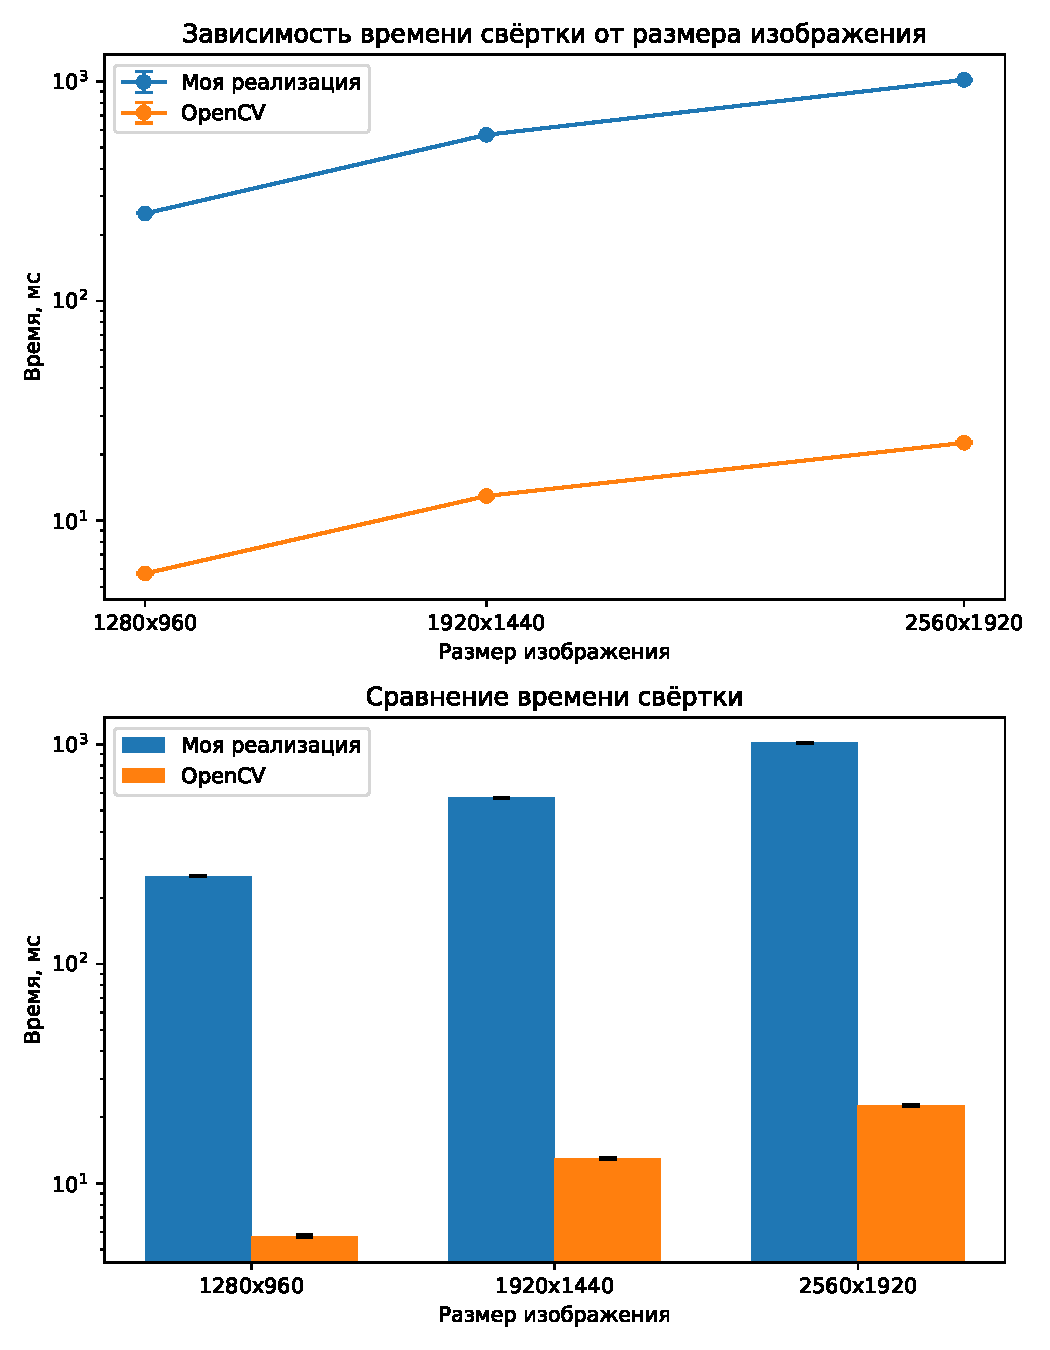
\includegraphics[width=0.85\textwidth]{plots.pdf}
    \caption{Зависимость среднего времени свёртки от размера изображения
    (сверху) и сравнение реализаций по размерам (снизу).
    Логарифмическая шкала по оси времени, отрезки~---
    доверительные интервалы 95\,\%.}
    \label{fig:plots}
\end{figure}

\textbf{Выводы из эксперимента.} OpenCV быстрее собственной реализации примерно в 44 раза, и это отношение почти не зависит от размера изображения. Постоянство ускорения ожидаемо: обе реализации имеют одинаковую асимптотическую сложность и отличаются лишь константой. Эта константа обусловлена оптимизациями OpenCV~--- векторизацией с помощью SIMD-инструкций процессора, эффективным использованием кеша и, для box blur, возможным разложением на два одномерных прохода (что уменьшает число операций). Эти приёмы уменьшают время в константное число раз, но не меняют порядок роста, поэтому отношение не зависит от размера. Время обеих реализаций растёт линейно с числом пикселей, что соответствует фиксированному числу операций на пиксель. Малая доля стандартного отклонения (1--4\,\% от среднего) говорит о стабильности измерений и косвенно~--- о достаточной стабильности среды. Доверительные интервалы корректны даже там, где формальные тесты на нормальность не проходят: при числе измерений около 40 этого достаточно для надёжной оценки среднего.

\section{Заключение}

В ходе выполнения работы получены следующие результаты:
\begin{itemize}
    \item выполнен обзор существующих решений и технологий; в качестве эталона и ориентира по скорости выбрана OpenCV;
    \item реализована двумерная свёртка RGB-изображений на языке~C с ядрами box blur, identity и Sobel и четырьмя режимами обработки границ, совпадающими по поведению с OpenCV;
    \item корректность подтверждена автоматическими тестами, сравнивающими результат с OpenCV на наборе изображений и всех режимах границ; тесты запускаются в CI;
    \item проведён эксперимент по сравнению производительности с OpenCV: показано, что OpenCV быстрее примерно в 44 раза независимо от размера, а время обеих реализаций растёт линейно с числом пикселей.
\end{itemize}

Репозиторий: \url{https://github.com/gorbuzova/convolution_rgb}

\end{document}
